%!TEX TS-program = xelatex
\documentclass[]{friggeri-cv}
\usepackage{afterpage}
\usepackage{hyperref}
\usepackage{color}
\usepackage{xcolor}
\usepackage{smartdiagram}
\usepackage{fontspec}
\usepackage{fontawesome}
\usepackage{metalogo}
\usepackage{dtklogos}
\usepackage[utf8]{inputenc}
\usepackage{tikz}
\usetikzlibrary{mindmap,shadows}
\hypersetup{
    pdftitle={},
    pdfauthor={},
    pdfsubject={},
    pdfkeywords={},
    colorlinks=false,
    allbordercolors=white
}
\smartdiagramset{
    bubble center node font = \footnotesize,
    bubble node font = \footnotesize,
    bubble center node size = 0.5cm,
    bubble node size = 0.5cm,
    distance center/other bubbles = 0.3cm,
    distance text center bubble = 0.5cm,
    bubble center node color = pblue,
    set color list = {lightgray, materialcyan, orange, green, materialorange, materialteal, materialamber, materialindigo, materialgreen, materiallime},
    bubble fill opacity = 0.6,
    bubble text opacity = 0.5,
}

\addbibresource{bibliography.bib}
\RequirePackage{xcolor}
\definecolor{pblue}{HTML}{0395DE}

\begin{document}
\header{Huynh Duc }{Dung}
      {Senior Full Stack Developer | AI Enthusiast}
      
\fcolorbox{white}{gray}{\parbox{\dimexpr\textwidth-2\fboxsep-2\fboxrule}{%
.....
}}

\begin{aside}
  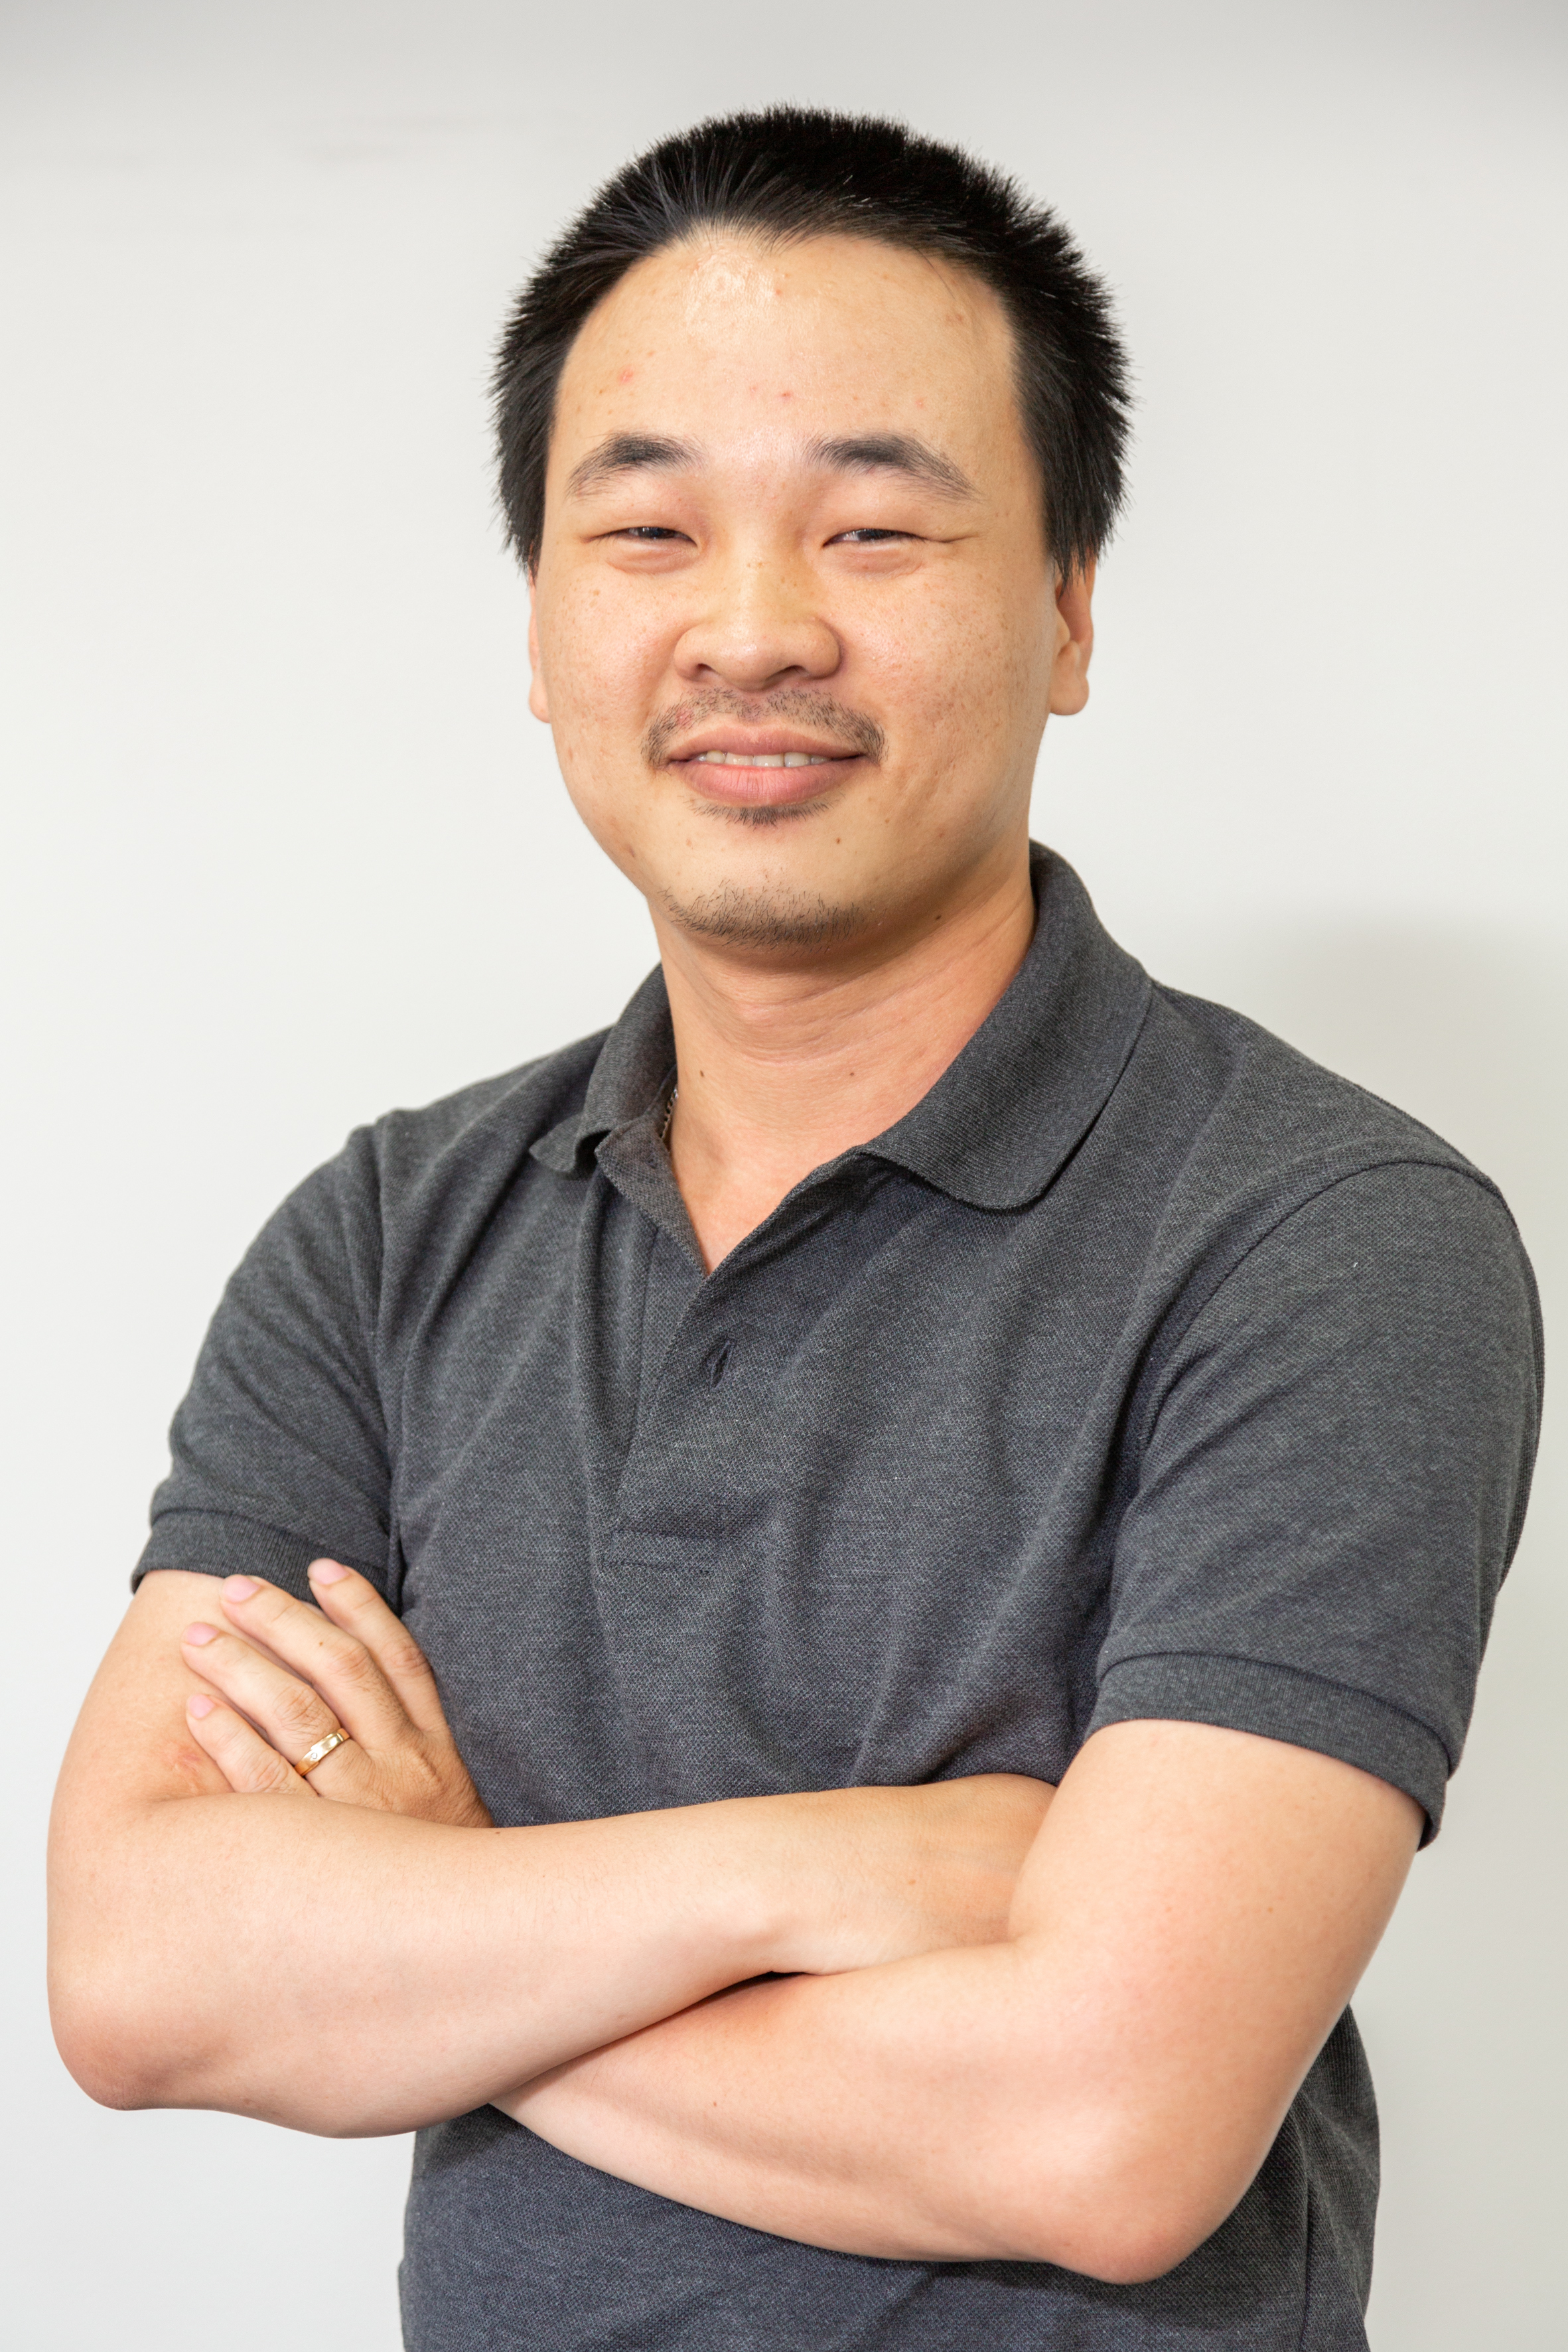
\includegraphics[scale=0.15]{img/Image-50.jpg}
  \section{Address}
   126 Lorong 1 Toa Payoh \#02-555 Singapore 310126
 \section{Nationality}
    Vietnam
    ~
  \section{Tel \& Skype}
    +65 89219468
    dunghd.it
    ~
  \section{Mail}
    \href{mailto:dunghd.it@gmail.com}{\textbf{dunghd.it@}gmail.com}
    ~
  \section{Web \& Git}
    \href{https://github.com/jellydn}{github.com/jellydn}
    \href{https://productsway.com/}{productsway.com}
    \href{https://blog.productsway.com/}{blog.productsway.com}
    ~
  \section{Programming}
    \smartdiagram[bubble diagram]{
        \textbf{Js/Typescript},
        \textbf{NodeJS},
        \textbf{ReactJS},
        \textbf{PHP}
    }
    ~
  \section{Personal Skills}
    \smartdiagram[bubble diagram]{
        \textbf{Problem}\\\textbf{Solving},
        \textbf{Independence},
        \textbf{Team}\\\textbf{Player},
        \textbf{Time}\\\textbf{Management},
        \textbf{\vspace{2mm}Leadership\vspace{2mm}},
        \textbf{Organize}
    }
    ~
\end{aside}
~
\section{About Me}
With over a decade of experience as a full-stack developer, I've had the opportunity to spearhead project teams at tech startups in Vietnam, Thailand, Japan, and Singapore. Additionally, I have worked as a freelance engineer for various companies based in Asia Pacific, Europe, and North America.

I currently hold the position of Senior Full Stack Software Engineer at AirCarbon and was one of the founding members of the tech team. My role involves developing advanced blockchain solutions using a microservices architecture with NodeJs, TypeScript, and ReactJs/NextJs. I lead the development of cutting-edge and scalable applications while staying current with the latest technologies.

I also publish a weekly video on the IT Man YouTube Channel every Sunday. You can find the videos at https://github.com/jellydn/itman-channel.

\section{Open Source Projects}
\textbf{Web Development:}
\begin{itemize}
    \item \textbf{NextJs Swagger Doc:} \href{https://github.com/jellydn/next-swagger-doc}{https://github.com/jellydn/next-swagger-doc}
    \item \textbf{Fastify Starter:} \href{https://github.com/jellydn/fastify-starter}{https://github.com/jellydn/fastify-starter}
    \item \textbf{NextJs App Starter:} \href{https://github.com/jellydn/next-app-starter}{https://github.com/jellydn/next-app-starter}
    \item \textbf{Moleculer TS Template:} \href{https://github.com/jellydn/moleculer-typescript-template}{https://github.com/jellydn/moleculer-typescript-template}
    \item \textbf{xBitly - URL Shortener:} \href{https://github.com/ProductsWay/xBitly}{https://github.com/ProductsWay/xBitly}
\end{itemize}

\textbf{Blockchain:}
\begin{itemize}
    \item \textbf{How to create your own NFT and mint NFT token:} \href{https://github.com/jellydn/nft-app}{https://github.com/jellydn/nft-app}
    \item \textbf{How to do your first ICO smart contract:} \href{https://github.com/jellydn/dapp-token-ico}{https://github.com/jellydn/dapp-token-ico}
\end{itemize}

\textbf{Real-time \& gRPC:}
\begin{itemize}
    \item \textbf{gRPC Demo Monorepo:} \href{https://github.com/jellydn/grpc-demo-monorepo}{https://github.com/jellydn/grpc-demo-monorepo}
\end{itemize}

\textbf{Rust Projects:}
\begin{itemize}
    \item \textbf{FB Seeder Tool:} \href{https://github.com/ProductsWay/fb-seeder-tool}{https://github.com/ProductsWay/fb-seeder-tool}
\end{itemize}

\textbf{Go Projects:}
\begin{itemize}
    \item \textbf{Simple interactive to install biome to your project:} \href{https://github.com/jellydn/biome-interactive}{https://github.com/jellydn/biome-interactive}
\end{itemize}

\textbf{AI \& Machine Learning:}
\begin{itemize}
    \item \textbf{GitHub Copilot Chat in Neovim:} \href{https://github.com/CopilotC-Nvim/CopilotChat.nvim}{https://github.com/CopilotC-Nvim/CopilotChat.nvim}
    \item \textbf{GPT-4 Free:} \href{https://github.com/jellydn/gpt4free-demo}{https://github.com/jellydn/gpt4free-demo}
    \item \textbf{Summary Chatbot:} \href{https://github.com/jellydn/summary-chatbot-demo}{https://github.com/jellydn/summary-chatbot-demo}
    \item \textbf{LLaMA2 Personal AI:} \href{https://github.com/jellydn/llama2-personal-ai}{https://github.com/jellydn/llama2-personal-ai}
    \item \textbf{Auto TestGen NodeJS:} \href{https://github.com/jellydn/auto-testgen-nodejs}{https://github.com/jellydn/auto-testgen-nodejs}
\end{itemize}


\newpage
\section{Experience}
\begin{entrylist}
    \entry
    {03/2020 - Now}
    {Sr. Full Stack Software Engineer}
    {AirCarbon Pte. Ltd.}
    {Working on a carbon exchange platform in Singapore using TypeScript and ReactJS. Responsible for full-stack development, microservices architecture, and cloud deployments.}
    \entry
    {09/2018 - 2/2020}
    {Lead Frontend Engineer}
    {Zenport Inc. (Logistics Startup)}
    {Led a small team of front-end developers in building a core logistics platform in Tokyo, Japan. Managed project timelines, code reviews, and implemented agile practices.}
  \entry
    {11/2017 - 6/2018}
    {Web Developer}
    {Zanroo (MarTech Startup)}
    {Developed web applications using NodeJS, TypeScript, and ReactJS. Contributed to the growth of the startup by delivering scalable solutions for marketing technologies.}
  \entry
    {07/2015 - 10/2017}
    {Freelancer}
    {Products Way/Upwork}
    {Worked on various startup projects for US, European, and Canadian clients. Specialized in NodeJS and PHP, focusing on backend development and API integrations.}
  \entry
    {05/2014 - 07/2015}
    {Lead Engineer}
    {Global Cybersoft}
    {Led a team for website projects targeting the Japanese market. Responsible for project management, client communication, and technical leadership.}
 \entry
    {12/2012 - 03/2014}
    {Deputy Manager}
    {Green Global}
    {Managed a mobile development team of 8 members. Led the development of Android and iOS applications, ensuring timely delivery and quality standards.}
  \entry
    {11/2013 - 01/2014}
    {Software Developer}
    {GMO Internet Group (On Site)}
    {Developed websites and iOS applications during an on-site business trip to Japan. Collaborated closely with Japanese clients to meet their specific requirements.} 
   \entry
    {8/2010 - 11/2012}
    {Developer/Team Lead}
    {Green Global}
    {Led the development of websites for Australian clients, utilizing modern web technologies and ensuring high standards of code quality.}
  \entry
    {11/2009 - 7/2010}
    {Developer (Part-time)}
    {CSSE}
    {Developed a website using the CodeIgniter framework, contributing to a project that enhanced the client’s digital presence.}
\end{entrylist}
\\
\section{Education}
\begin{entrylist}
  \entry
    {2006 - 2011}
    {Bachelor's Degree in Software Engineering}
    {Danang University of Technology}
    {Graduated with a GPA of 7.4/10. Gained a strong foundation in software development, algorithms, and data structures.}
\end{entrylist}

\newpage

\begin{aside}
~
~
~
  \section{OS Preference}
    \textbf{MacOS}\includegraphics[scale=0.40]{img/5stars.png}
    \textbf{GNU/Linux}\includegraphics[scale=0.40]{img/4stars.png}
    \textbf{Unix}\includegraphics[scale=0.40]{img/4stars.png}
    \textbf{Windows}\includegraphics[scale=0.40]{img/3stars.png}
    ~
  \section{Languages}
    \textbf{Vietnamese}\includegraphics[scale=0.40]{img/5stars.png}
    \textbf{English}\includegraphics[scale=0.40]{img/4stars.png}
    ~
\end{aside}

\section{AWARD, ACHIEVEMENT}
\includegraphics[scale=0.40]{top-rated.png}
\emph{Top rated developer on Upwork since 2016.\\}
\emph{Promoted to Deputy Manager at Green Global in 2013.\\}
\emph{Employee of the Year at Green Global in 2012.\\}
\emph{IT Club Staff Member in 2011.\\}
\emph{Leader of the Soft Skill Club in 2010.}
\\
\begin{flushleft}
\emph{August 16th, 2024}
\end{flushleft}
\begin{flushright}
\emph{Huynh Duc Dung}
\end{flushright}

\end{document}